\chapter{Numerical methods and validation}
\label{ch:numerics}

\newcommand{\valoneBlockA}{702.2}
\newcommand{\valoneBlockErrA}{2.5}
\newcommand{\valoneBlockMinA}{697}
\newcommand{\valoneBlockMaxA}{706}
\newcommand{\vallargeA}{6.20}
\newcommand{\vallargeErrA}{0.02}
\newcommand{\valoneBlockB}{700.8}
\newcommand{\valoneBlockErrB}{2.4}
\newcommand{\valoneBlockMinB}{697}
\newcommand{\valoneBlockMaxB}{705}
\newcommand{\vallargeB}{6.20}
\newcommand{\vallargeErrB}{0.03}
\newcommand{\valerrCascadeHA}{9.3e-08}
\newcommand{\valstatEventsA}{1{,}000{,}000}
\newcommand{\valstatEventsB}{1{,}000{,}000}


This chapter describes how the models of the previous chapters are simulated and how we know that the programs are
correct. The guiding principle is that no simulation result is used unless the program that produced it has first
reproduced known results: exact solutions, conservation laws, and an independent reference implementation. We describe
the software (\cref{sec:num-software}), the algorithms for the sandpile (\cref{sec:num-btw}), the BK model
(\cref{sec:num-bk}) and its sandpile limit (\cref{sec:num-mapped}), and the tests that each of them passes. The last
section (\cref{sec:num-legacy}) lists the errors found in the earlier version of this project, which motivated the complete
rewrite.

% ======================================================================
\section{Software}
\label{sec:num-software}

All programs are written in Python. The time-critical loops are compiled to machine code with Numba, which gives the speed of
C while keeping the code readable. The code is organised as a small package, \code{bksoc}, with one module per model:
\begin{center}
\begin{tabular}{@{}ll@{}}
\toprule
module & content \\
\midrule
\code{sandpile.py} & BTW sandpile on an arbitrary lattice (Chapter~\ref{ch:soc}) \\
\code{theory.py} & exact results for Abelian sandpiles, used as test references \\
\code{stats.py} & binning, maximum-likelihood fits, blocking, finite-size scaling (Chapter~\ref{ch:measuring}) \\
\code{bk.py} & Burridge--Knopoff chain (Chapter~\ref{ch:bk}) \\
\code{mapped.py} & sandpile limit of the BK chain (Chapter~\ref{ch:mapping}) \\
\bottomrule
\end{tabular}
\end{center}
Each figure of this thesis is produced by a script in \code{scripts/thesis/}, which runs the simulations, stores the raw results
together with a file of parameters and random seeds, and draws the figure; the numbers quoted in the text are written by the same
scripts. The test suite, \code{tests/}, contains 81 tests and runs in about a minute and a half. A single simulation always runs on one
processor core; independent runs (different parameters or seeds) are distributed over the cores of the machine. This is far more
efficient than parallelising one run, because the dynamics of an avalanche or an event is inherently sequential.

% ======================================================================
\section{The sandpile}
\label{sec:num-btw}

\paragraph{Algorithm.} The lattice is stored as a table of neighbours: row $i$ lists the $k$ neighbour slots of site $i$, and a slot
pointing outside the lattice is marked with $-1$. This one representation covers chains, square lattices and any other graph. An
avalanche is relaxed with the parallel update of \cref{sec:btw-def}: a list holds the sites that are unstable at the start of a time
step, all of them topple, and the sites made unstable by this are collected into the list for the next step. Each toppling costs a fixed
number of operations, so the cost of an avalanche is proportional to its size; on one core the program performs about $4\times10^7$
topplings per second.

\paragraph{Validation.} The tests check, in order of increasing strength:
\begin{itemize}[nosep]
  \item conservation of grains (grains added $=$ grains in the system $+$ grains lost);
  \item the Abelian property, by comparing every avalanche with an independent, slow implementation that topples unstable sites one at a
    time in \emph{random} order (same final configuration, size and area);
  \item the exact one-dimensional solution of \cref{sec:btw1d}, for every recurrent configuration and every seed, including the full
    toppling profile \cref{eq:n1d};
  \item the stationary size distribution of the chain, against the exact enumeration, with a $\chi^2$ test;
  \item the number of recurrent configurations, $\det\Delta$, by counting the states visited in a long run;
  \item the exact mean avalanche size \cref{eq:mean-s} and the height probabilities of the two-dimensional model (\cref{sec:btw2d}).
\end{itemize}

% ======================================================================
\section{The Burridge--Knopoff chain}
\label{sec:num-bk}

\subsection{The difficulty}

\Cref{eq:bk} is an ordinary differential equation, but not a smooth one: the friction force jumps when a block starts or stops slipping,
and a stuck block is not described by an equation of motion at all but by a constraint. Standard integrators with a fixed time step handle
such switches poorly. If a stop or a start is noticed only at the end of a time step, the error made in that step is proportional to the
step size $h$, whatever the order of the integrator. Since a large event contains thousands of such switches, they dominate the error.

\subsection{Algorithm}

The program treats stuck and slipping blocks separately.
\begin{enumerate}
  \item \textbf{Loading.} Between events all blocks are stuck. The program finds the block with the largest force $f_j$ and moves the plate
    exactly far enough that this force reaches 1 (for $\nu=0$; for $\nu>0$ the time advances by the corresponding amount). The block becomes
    \emph{active}.
  \item \textbf{Integration.} Only active (slipping) blocks are integrated, with the classical fourth-order Runge--Kutta method; stuck blocks
    stay exactly at rest. The cost of a time step is therefore proportional to the number of slipping blocks, not to $N$.
  \item \textbf{Stopping.} When the velocity of a slipping block changes sign during a step, the block sticks. Its position is corrected to the
    moment of the zero crossing, assuming constant acceleration within the step: if the velocity went from $V_0>0$ to $V_1\le0$, the crossing
    happened after a fraction $\theta = V_0/(V_0-V_1)$ of the step, and the block is placed at $U_0 + \tfrac12V_0\theta h$.
  \item \textbf{Starting.} After each step the program checks whether a stuck block has reached the threshold. If so, the moment of crossing is
    found by linear interpolation of its force between the beginning and the end of the step, and the block starts with the velocity and
    displacement it would have gained since that moment. This correction is what makes the method second-order accurate (see below).
  \item \textbf{Events.} An event is a cluster of slip that is connected in space and time. A block that starts to slip while one of its neighbours is
    slipping (or stopped in the same time step) joins that neighbour's event; otherwise it starts a new event, and two events that come into contact
    are merged. An event is over when its last block sticks. The program then records its moment, the number of distinct blocks that slipped, its
    duration, its epicentre, the plate position, and the energy dissipated by friction. For $\nu = 0$ the plate is frozen while blocks slip, so only
    one event can exist at a time and this definition reduces to ``everything between two loadings of the plate''. For $\nu>0$ several events can
    coexist in different parts of the chain, as in the simulations of Carlson and Langer (1989).
\end{enumerate}
With the 1989 friction law, a block whose velocity returns to zero while its force is still outside the static range simply starts again; following
Carlson and Langer, each such return of the velocity to zero ends one slip episode, so that the periodic small slips of a slowly creeping block are
counted as separate one-block events.
To find the block closest to the threshold without scanning all $N$ blocks, the forces of the stuck blocks are kept in a \emph{segment tree}, a
binary tree in which every node stores the largest value below it. Updating one force and finding the largest one both take a time proportional to
$\log N$. With these choices a chain of 4096 blocks runs at about $4\times10^4$ events per second; one unit of plate displacement takes between
0.2 seconds ($\ell=6$, $\alpha=3$) and a few seconds ($\ell=14$, $\alpha=1$, $N=8192$), because events are larger and last longer for stiffer chains and
weaker velocity weakening.

\paragraph{Time step.} The fastest motion in the chain is its highest normal mode, with angular frequency $\omega_{\max} = \sqrt{4\ell^2+1}$ (neighbouring
blocks moving in opposite directions). We use $h = 0.1/\omega_{\max}$, i.e.\ about 60 steps per period of the fastest oscillation.

\subsection{Validation}

\paragraph{Exact one-block events.} An isolated block reaching the threshold in a stuck chain must slip by $2\sigma/(2\ell^2+1)$ when velocity weakening is
switched off (\cref{eq:dU1}). The program reproduces this to seven significant digits, and the duration $\pi/\omega_1$ to the accuracy of the time step. With
velocity weakening it agrees with the solution of the single-block equation with the full nonlinear friction law to $10^{-4}$, and with the linearised
formula \cref{eq:dU1-alpha} to 2\%.

\paragraph{Comparison with a reference solver.} The most demanding test compares whole events with an independent implementation. The reference solver
integrates the equations of motion with an adaptive high-order method (Dormand--Prince of order 8, relative tolerance $10^{-11}$) and locates every stop and
every start exactly, by root finding on the velocity of each slipping block and on the force of each stuck block; between two such switches the set of slipping
blocks is fixed and the equations are smooth. The comparison uses chains of ten blocks prepared so close to threshold that the event cascades through all of
them. \Cref{fig:convergence} shows the largest difference in the final positions as a function of the time step: it decreases as $h^2$, and at $h=10^{-3}$ it is
$\valerrCascadeHA$, for slips of order one. During the development of the program, before the starting correction (item 4 above) was introduced, the same test
showed only first-order convergence, with errors about a thousand times larger.

\begin{figure}[t]
  \centering
  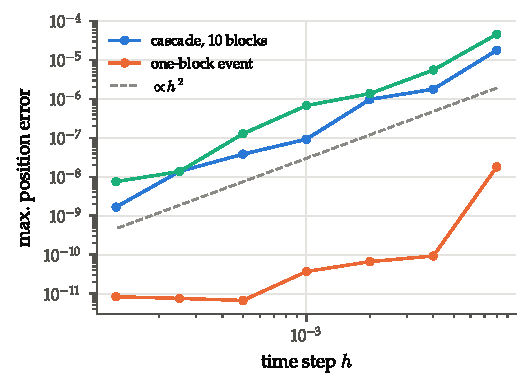
\includegraphics[width=0.58\linewidth]{validation/convergence.pdf}
  \caption{Error of the BK program against the reference solver, for single events in a chain of ten blocks. For one-block events the error reaches the tolerance of
  the reference solver.}
  \label{fig:convergence}
\end{figure}

\paragraph{Conservation laws.} With the plate at rest, the mechanical energy (kinetic energy plus the elastic energy of all springs) lost in an event must equal the
work done by friction, which the program accumulates with the same Runge--Kutta weights as the motion. Over thousands of events the two agree with a median relative
difference of $3\times10^{-7}$. The total moment of all events equals $N$ times the increase of the mean block position to machine precision, and the mean block
position stays within a bounded distance of the plate, as the sum rule requires.

\paragraph{Invariances.} No block ever moves backwards with the 1991 law, all forces are below the threshold after every event, the result is unchanged when the chain
is mirrored, and shifting all blocks and the plate by the same amount leaves the events unchanged. (In the last test only the first events are compared: the model is
chaotic, and differences of the order of the rounding error, $10^{-15}$, eventually grow to visible size.)

\paragraph{The 1989 friction law.} The reference solver was extended to the symmetric friction law, with backward slip and a moving plate. Whole cascades in
chains of eight blocks agree with it to $10^{-4}$ in the final positions. A block that reaches the threshold in a slowly loaded chain creeps with an
oscillating velocity; its first slip episode, of size about $2\pi\nu/\omega_1^3$, agrees with the exact single-block solution to $2\times10^{-3}$. This last
test exposed an error in an intermediate version of the program: within a Runge--Kutta step, a stage velocity slightly below zero made the symmetric friction
change sign and gave the block a spurious kick, so that creeping blocks ``bounced'' instead of stopping. Friction is now always evaluated against the current
direction of motion. Further tests check that every slip is assigned to an event (the moments of completed and unfinished events add up to the total slip
exactly), that no event is left unrecorded once all its blocks have stopped, that the number of blocks in an event never exceeds $N$, and that two blocks
reaching the threshold at the same time far apart produce two separate events. For a single block, the slip of each stick--slip cycle agrees with a direct
integration to $10^{-3}$.

\paragraph{Statistical convergence.} Because the dynamics is chaotic, individual trajectories computed with different time steps eventually diverge, and convergence must
be checked on the statistics. \Cref{fig:statistical} compares the distribution $\mathcal D(\mu)$ for $h = 0.1/\omega_{\max}$ and $h=0.05/\omega_{\max}$ ($N=1024$, $\ell=6$,
$\alpha=3$, $\sigma=0.01$, $10^6$ events each). The two curves are indistinguishable by eye, but a quantitative comparison taught us something about the errors. For all
magnitudes except the smallest the two runs agree within their statistical errors; the rate of one-block events, which make up 85\% of all events, differed by 2\%, many
times its error estimated by blocking the time series into 50 pieces. To decide whether this was an effect of the time step, we repeated the runs with three independent
initial conditions for each time step (600 units of plate displacement each). The rate of one-block events per unit plate displacement varies between runs from
$\valoneBlockMinA$ to $\valoneBlockMaxA$ for the larger step and from $\valoneBlockMinB$ to $\valoneBlockMaxB$ for the smaller one; the averages, $\valoneBlockA\pm\valoneBlockErrA$
and $\valoneBlockB\pm\valoneBlockErrB$, agree, as do the rates of large events ($M>6$), $\vallargeA\pm\vallargeErrA$ and $\vallargeB\pm\vallargeErrB$. The time step
therefore has no detectable effect on the statistics. The difference seen in the first comparison is a run-to-run fluctuation: the rate of small events depends on the
slowly evolving roughness of the chain, whose memory is longer than the blocks used in the first error estimate. For quantities of this kind we estimate errors from
independent runs.

\begin{figure}[t]
  \centering
  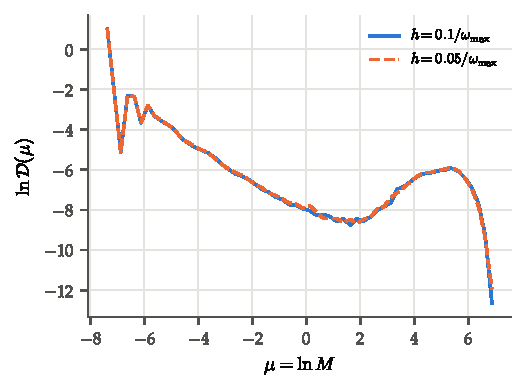
\includegraphics[width=0.58\linewidth]{validation/statistical.pdf}
  \caption{Distribution of event magnitudes of the BK model computed with two time steps.}
  \label{fig:statistical}
\end{figure}

% ======================================================================
\section{The sandpile limit}
\label{sec:num-mapped}

The program for the sandpile limit of Chapter~\ref{ch:mapping} combines the two previous ones: the forces $f_j$ are relaxed with the parallel update of the sandpile,
and the plate is moved as in the BK program, with a segment tree to find the next block to reach the threshold. It performs between $5\times10^5$ and $10^6$ avalanches per
second for the chains used here. The tests check that the fixed-drop rule is Abelian (against a random-order reference implementation), that the force bookkeeping
\cref{eq:force-bookkeeping} holds to rounding precision, that all forces are below the threshold after every avalanche, that an isolated toppling with the drop
\cref{eq:map-drop} reproduces the one-block event of the BK program, that changing the drop only changes the unit of slip, and that threshold noise breaks the
periodicity without violating the force bookkeeping.

% ======================================================================
\section{Statistical tools}
\label{sec:num-stats}

The methods of Chapter~\ref{ch:measuring} are tested on synthetic data with known answers: the maximum-likelihood estimates (continuous, discrete and truncated) recover
the exponents used to generate the data within their error bars, and the error bars themselves are correct (68\% coverage); the discrete sampler reproduces the exact
probabilities; the choice of $x_{\min}$ finds the onset of a power-law tail; the goodness-of-fit test accepts a power law and rejects an exponential; the blocking
method reproduces the exact error of the mean of a correlated (autoregressive) process; and the moment analysis and data collapse recover the exponents of synthetic
finite-size-scaling data, including the exact corrections to scaling.

% ======================================================================
\section{The earlier implementation}
\label{sec:num-legacy}

The earlier version of this project did not reproduce the results of Carlson and Langer. A review of its code, carried out before the rewrite, found the following
problems. They are listed because each of them is a mistake that is easy to make and hard to notice without tests of the kind described above.
\begin{enumerate}
  \item \textbf{An error in the Runge--Kutta step.} The fourth stage used $v + \tfrac12k_3$ instead of $v + h\,k_3$ for the velocity, so the integration was not of
    fourth order; in fact it was not consistent at all for the positions.
  \item \textbf{Stiffness tied to the system size.} The pulling-spring constant was set to $k_p = 1/(L-1)$, with $L$ the number of blocks, so that changing the length of
    the chain also changed the stiffness ratio $\ell^2$.
  \item \textbf{Units.} The program used units in which $k_c = m = F_0 = 1$, while the friction parameter was compared directly with the $\alpha$ of the papers. As shown in
    \cref{sec:bk-units}, a friction coefficient $c$ in such units corresponds to $\alpha = c/(2\sqrt{k_p})$, e.g.\ $\alpha=2.5\,c$ for $k_p = 0.04$.
  \item \textbf{Boundary conditions.} The missing neighbours of the end blocks were set to zero displacement, which attaches the chain to fixed walls, instead of the free ends
    of the papers.
  \item \textbf{Stick--slip handling.} The friction law was evaluated inside the Runge--Kutta stages with the static or kinetic branch chosen from intermediate velocities,
    and negative velocities were simply set to zero at the end of each step, without locating the stopping time. Starts of slip were detected only at the end of a step.
  \item \textbf{Event durations.} In the GPU version the array of times was never filled, so all event durations were recorded as zero.
\end{enumerate}
Each of these would be caught immediately by one of the tests of \cref{sec:num-bk}: the one-block event, the comparison with the reference solver, or the energy balance.
